<<<<<<< HEAD
\section{Research Gaps}
\label{sec:RG}

Resilience is now a routine demand in policy documents, strategy discussions, and academic work, yet it remains difficult to use analytically in organizational settings. The problem is not that the literature is thin. It is the opposite. Engineering, ecology, psychology, and complex systems have all produced substantial work on resilience, but they are not describing the same phenomenon and they do not proceed from the same assumptions. Most of these traditions were not developed for organization-level analysis in the first place. Once resilience is imported into managerial and regulatory settings, that divergence stops being an abstract theoretical issue and becomes a practical one. Organizations are asked to demonstrate resilience, yet they are given limited clarity about what that should mean in practice, how it should be measured, or how it should be governed \autocite{hillmann2021organizational}.\\

Part of the problem is semantic, but only part. Across disciplines, resilience has been used to refer to recovery, robustness, adaptation, learning, and transformation. These labels are often treated as adjacent, sometimes even as interchangeable, yet they rest on different views of time, change, and system behavior. A recovery-oriented account assumes that disruption is followed by return. A transformative account does not. It allows for the possibility that disruption changes the system more fundamentally. When these perspectives are carried into organizational settings, they do not produce the same priorities. A firm may invest in robustness and then be evaluated on adaptability, or build compliance structures while being told it should become more transformative.\\

This review argues that three related problems follow from that situation: conceptual plurality without operational convergence, limited empirical validation of adaptive performance, and methodological fragmentation across domains. The first problem is conceptual. Management and information systems research still lacks a shared operational core for studying resilience. The second is empirical. Resilience is rarely examined through direct observation of how organizations adapt over time. The third is methodological. Existing metrics and formal models remain only weakly connected to the governance and evaluation systems organizations actually use. Of these, the issue of operationalizable and transferable measures is especially important \autocite{woods2015four}. Similar concerns have been raised in fields such as infrastructure and healthcare \autocite{heinimann2017infrastructure,kruk2017building}. Details of the review process are reported in Appendix~\ref{appendix:B}, and Appendix~\ref{appendix:C} summarizes how these tensions appear in organizational practice.\\
\\
First, \textbf{conceptual plurality without operational convergence}. Resilience has been conceptualized through lenses of mechanical stability, ecological transformation, cognitive adaptability, and socio-technical flexibility (see Appendix~\ref{appendix:A}). Each of these perspectives offers useful and often rigorously developed insights, but their assumptions are not equivalent. Engineering resilience emphasizes restoration of predefined functions. Ecological resilience foregrounds regime shifts and adaptive reorganization. Psychological resilience centers on coping, endurance, and growth under stress. Socio-technical perspectives highlight emergence, interdependence, and distributed coordination. These perspectives can be read as complementary at a high level, but their implications for organizational design, measurement, and accountability differ substantially.\\

In organizational practice, this plurality often turns into definitional drift. Terms such as resistance, robustness, recovery, agility, and adaptation are frequently used as though they referred to the same thing, even when they point to different mechanisms and temporal dynamics. As a result, resilience is often invoked symbolically through strategy documents, audits, or compliance templates rather than embedded as a coherent adaptive capability \autocite{duchek2020organizational}. Without a clearer account of how these perspectives translate into observable organizational mechanisms, resilience risks remaining conceptually rich while operationally diffuse.\\
\\
Second, \textbf{limited empirical validation and longitudinal grounding}. Empirical studies in cybersecurity and risk management suggest that resilience is usually assessed through compliance artifacts such as audits, maturity models, and certifications rather than through systematic observation of adaptive performance during disruption. More advanced tools, including predictive simulations and anomaly detection, are sometimes piloted in innovation units, but they remain weakly integrated into regulatory evaluation structures \autocite{skopik2016problem}. At the same time, informal practices such as parallel communication channels, crisis improvisation, and decentralized escalation often prove crucial to adaptive response, yet remain largely invisible within existing assessment frameworks.\\

The same mismatch appears in healthcare and public health systems. Resilience is often practiced there, but only partially built into measurement frameworks \autocite{kruk2017building}. Longitudinal studies tracing how resilience evolves across repeated disruptions remain relatively rare. Few frameworks directly address the uncertainty, reversibility, and trade-offs involved in resilience assessment \autocite{allen2018quantifying}. Disciplinary fragmentation compounds the problem. Analytical methods developed in control theory or complex systems rarely migrate into organizational research, while widely used practices such as awareness campaigns often fail to produce measurable behavioral adaptation \autocite{bada2019cyber}.
\\
To examine how resilience research is distributed across domains and methodological approaches, we systematically classified 89 publications according to thematic focus and analytical method. The resulting cross-disciplinary map (Table~\ref{tab:ResearchGaps}) shows clear asymmetries in how resilience is studied, particularly the limited use of quantitative markers, metrics, and simulation approaches within organizational and managerial contexts.\\
\\
\begin{center}
\newgeometry{top=.15cm, bottom=2cm, left=2.3cm, right=2.3cm}
\singlespacing
\begin{landscape}
\tiny
\begin{longtblr}[
  caption = {\textbf{Classification of Resilience-related Publications.} This table provides the classification of 89 relevant, impactful and supporting publications associated with resilience according to their corresponding topic/-s and used methodology/-ies. This table allows to extract the key research gaps, where no publication was found (red cells) or only very few (orange cell). Topic-methodology intersections in grey show other research that are less relevant for this research.},
  label = {tab:ResearchGaps}
]{
  width=\linewidth,
  colspec={|Q[1.5cm] Q[1.7cm]|Q[2.6cm] Q[2.6cm] Q[2.6cm] Q[2.6cm] Q[2.6cm] Q[2.6cm] Q[2.6cm]|},
  rowhead = 2,
  hlines, vlines
}
\SetCell[r=2, c = 2]{l} \vspace{2em}\par \textit{Topics}& & \SetCell[r = 1, c = 7]{halign = l}{\textit{Methodologies}} \\
& & \textbf{\makecell{Simulation \\ \& \\ Modeling}} & \textbf{\makecell{Network \\ Analysis}} & \textbf{\makecell{Markers \\ \& \\ Metrics}} & \textbf{\makecell{Technology}} & \textbf{\makecell{Case Studies}} & \textbf{\makecell{Longitudinal \\ Studies}} & \textbf{\makecell{Surveys}} \\
\hline
% === Example block start ===
\SetCell[r=1, c=2]{l}{\textbf{\makecell{Complex Adaptive Systems}}} & &  \SetCell[r=1, c = 1]{l} {\cite{holling1973resilience} \\ \cite{gao2016universal} \\ \cite{pumpuni2017resilience} \\ \cite{krakovska2023resilience}} & \SetCell[r=1, c = 1]{l}{\cite{albert2000error} \\ \cite{bodin2009role} \\ \cite{gao2016universal} \\ \cite{pumpuni2017resilience}} & \SetCell[r=1, c = 1]{l} {\cite{anderies2004framework} \\ \cite{sundstrom2014transdisciplinary} \\ \cite{pumpuni2017resilience}} & \SetCell[r=1, c = 1]{bg = gray!50} & \SetCell[r=1, c = 1]{l} {\cite{ostrom1990governing} \\ \cite{lanzara1999transient} \\ \cite{folke2004regime} \\ \cite{weick2011managing}} & \SetCell[r=1, c = 1]{bg = gray!50} & \SetCell[r=1, c = 1]{l}{\cite{ostrom1990governing} \\ \cite{levin1998ecosystems} \\ \cite{gunderson2002panarchy} \\ \cite{walker2004resilience} \\ \cite{heinimann2017infrastructure}}\\
\hline
\SetCell[r=1,c=2]{l}{\textbf{\makecell{Engineering}}} & & \SetCell[r=1, c = 1]{l}{\cite{wiener1948cybernetics} \\ \cite{panteli2017metrics}} & \SetCell[r=1, c = 1]{l}{\cite{albert2000error} \\ \cite{gao2016universal}} & \SetCell[r=1, c = 1]{l}{\cite{bruneau2003framework} \\ \cite{francis2014metric} \\ \cite{panteli2017metrics}} & \SetCell[r=1, c = 1]{l}{\cite{rane2024artificial}} & \SetCell[r=1, c = 1]{l}{\cite{paries2017resilience}} & \SetCell[r=1, c = 1]{bg = gray!50} & \SetCell[r=1, c = 1]{l}{\cite{holling1996engineering} \\ \cite{francis2014metric} \\ \cite{ivanov2022viable}} \\
\hline
\SetCell[r=1,c=2]{l}{\textbf{\makecell{Ecology \& Social Systems}}} & & \SetCell[r=1, c = 1]{l}{\cite{holling1973resilience} \\  \cite{hashimoto1982reliability} \\ \cite{ives1995measuring}} & \SetCell[r=1, c = 1]{l}{\cite{bodin2009role}} & \SetCell[r=1, c = 1]{l}{\cite{ives1995measuring} \\ \cite{sundstrom2014transdisciplinary}} & \SetCell[r=1, c = 1]{l}{\cite{maillart2024computational}} & \SetCell[r=1, c = 1]{l}{\cite{berkes1998linking} \\ \cite{lebel2006governance} \\ \cite{mahajan2022participatory}} & \SetCell[r=1, c = 1]{l}{\cite{maillart2024computational}} & \SetCell[r=1, c = 1]{l}{\cite{folke2010resilience} \\ \cite{leslie2013response}\\ \cite{francis2014metric} \\ \cite{allen2018quantifying}}\\
\hline
\SetCell[r=1,c=2]{l}{\textbf{\makecell{Climate Change \& Disaster Management}}} & & \SetCell[r=1, c = 1]{l}{\cite{dawson2011agentbased} \\ \cite{panteli2017metrics} \\ \cite{aydin2018integration}} & \SetCell[r=1, c = 1]{l}{\cite{jacobs2017applying} \\ \cite{aydin2018integration}} & \SetCell[r=1, c = 1]{l}{\cite{bruneau2003framework}} & \SetCell[r=1, c = 1]{l}{\cite{arnold2004informationsharing} \\ \cite{aerts2018integrating}} & \SetCell[r=1, c = 1]{l}{\cite{dawson2011agentbased} \\ \cite{mahajan2022participatory}} & \SetCell[r=1, c = 1]{l}{\cite{moreno2018womens}} & \SetCell[r=1, c = 1]{l}{\cite{alexander2013resilience} \\ \cite{meerow2016defining} \\ \cite{adger2005socialecological} \\ \cite{leichenko2024climate}}\\
\hline
\SetCell[r=1,c=2]{l}{\textbf{\makecell{Psychology \& Neuroscience}}} & & \SetCell[r=1, c = 1]{l}{\cite{manikis2019computational} \\ \cite{ungar2021modeling}} & \SetCell[r=1, c = 1]{bg = gray!50} & \SetCell[r=1, c = 1]{l}{\cite{mcewen2004protection} \\ \cite{rakesh2019resilience}} & \SetCell[r=1, c = 1]{l}{\cite{klein2008performing} \\ \cite{bada2019cyber} \\\cite{kalisch2024neurobiology}} & \SetCell[r=1, c = 1]{l}{\cite{bada2019cyber}} & \SetCell[r=1, c = 1]{l}{\cite{rutter1987psychosocial} \\ \cite{masten2010disasters}} & \SetCell[r=1, c = 1]{l}{\cite{wagnild1993development} \\ \cite{luthar2000construct} \\ \cite{campbell2007psychometric} \\ \cite{feder2019biology}}\\
\hline
\SetCell[r=1,c=2]{l}{\textbf{\makecell{Public Health}}} & & \SetCell[r=1, c = 1]{l}{\cite{brauer2008compartmental} \\ \cite{luke2012systems}}  & \SetCell[r=1, c = 1]{l}{\cite{luke2012systems}} & \SetCell[r=1, c = 1]{l}{\cite{cutter2010disaster} \\ \cite{kruk2017building}} & \SetCell[r=1, c = 1]{l}{\cite{arnold2004informationsharing}} & \SetCell[r=1, c = 1]{l}{\cite{barasa2018what} \\ \cite{haldane2021health}} & \SetCell[r=1, c = 1]{l}{\cite{gibbs2013beyond} \\ \cite{aase2020resilience}} & \SetCell[r=1, c = 1]{l}{\cite{norris2007community} \\ \cite{barasa2018what}}\\
\hline
\SetCell[r=2, c=1]{l}{\vspace{-16.25em}\par \textbf{Management}} & \SetCell[r=1, c=1]{l}{\textbf{Organizational}} & \SetCell[r=1, c = 1]{bg = red!20} & \SetCell[r=1, c = 1]{bg = red!20} & \SetCell[r=1, c = 1]{l}{\cite{kuypers2018designing}} & \SetCell[r=1, c = 1]{l}{\cite{klein2008performing} \\ \cite{bada2019cyber} \\ \cite{almeida2020challenges}} & \SetCell[r=1, c = 1]{l}{\cite{lanzara1999transient} \\ \cite{westrum2004typology} \\ \cite{weick2011managing} \\ \cite{henfridsson2013generative} \\ \cite{barasa2018what} \\ \cite{bada2019cyber} \\\cite{boh2023building}} & \SetCell[r=1, c = 1]{bg = gray!50} &  \SetCell[r=1, c = 1]{l}{ \cite{westrum2004typology}\\ \cite{teece2007explicating} \\ \cite{vogus2007organizational} \\ \cite{bhamra2011resilience} \\ \cite{burnard2011organisational} \\ \cite{lengnick2011developing} \\ \cite{boin2013resilient} \\ \cite{henfridsson2013generative} \\ \cite{skopik2016problem} \\ \cite{dupont2019cyberresilience} \\ \cite{barasa2018what} \\ \cite{duchek2019organizational} \\ \cite{calder2021iso} \\\cite{hepfer2022heterogeneity} \\ \cite{he2022building}}\\
\cline[dashed]{2-9}
&  \SetCell[r=1, c=1]{l}{\textbf{Risk \& Cyber}} & \SetCell[r=1, c = 1]{bg = red!20} & \SetCell[r=1, c = 1]{bg = orange!20}{\cite{gillard2023efficient}} & \SetCell[r=1, c = 1]{l}{\cite{linkov2013resilience} \\ \cite{panteli2017metrics}} & \SetCell[r=1, c = 1]{l}{\cite{aerts2018integrating} \\ \cite{almeida2020challenges}} & \SetCell[r=1, c = 1]{l}{\cite{lostri2022shared} \\ \cite{boh2023building}} & \SetCell[r=1, c = 1]{l}{\cite{kuypers2018designing}} & \SetCell[r=1, c = 1]{l}{\cite{baselcommittee2011basel} \\ \cite{bjorck2015cyber} \\ \cite{woods2015four} \\ \cite{skopik2016problem} \\ \cite{linkov2019fundamental} \\ \cite{dupont2019cyberresilience} \\  \cite{hausken2020cyber}  \\ \cite{calder2021iso} \\ \cite{lostri2022shared}} \\
\end{longtblr}
\end{landscape}
\end{center}
\restoregeometry



Third, \textbf{methodological fragmentation and limited transfer}. This gap becomes especially visible in the cross-disciplinary classification of the 89 resilience-related publications summarized in Table~\ref{tab:ResearchGaps}. Simulation models, network analyses, and quantitative resilience metrics are well established in engineering, complex systems, and climate research \autocite{francis2014metric}. Their systematic integration into domains central to organizational and managerial resilience, such as cybersecurity, risk management, and strategic governance, remains much more limited. Table~\ref{tab:ResearchGaps} shows that \textit{Markers \& Metrics} and \textit{Technology} are comparatively underrepresented in these fields, and that simulation-based approaches are rarely incorporated into organization-level governance frameworks \autocite{linkov2013resilience,kuypers2018designing}. The result is continued reliance on maturity models, expert judgment, or audit documentation: approaches that may support compliance, but rarely capture adaptive performance under real-world conditions.\\

Even within cybersecurity, formal models of attack--defense dynamics exist \autocite{aydin2018integration}, yet they are seldom integrated into broader organizational resilience architectures. Other transferable approaches, including ecological network analysis \autocite{luke2012systems}, transportation recovery modeling \autocite{jacobs2017applying}, and agent-based infrastructure risk models \autocite{dawson2011agentbased}, also remain underused in digital resilience planning. The problem is therefore not methodological scarcity. It is the weak translation of technical advances in resilience measurement into governance tools that organizations can actually use \autocite{heinimann2017infrastructure,aerts2018integrating}.\\
\\
These gaps do not remain separate. They reinforce one another. Conceptual plurality complicates measurement. Limited empirical validation weakens cumulative evidence. Methodological fragmentation restricts the transfer of analytical tools across domains. As a result, resilience research contains substantial theoretical and methodological resources, but still lacks sufficient integration to support cumulative, organization-ready application. Without standardized, validated, and scalable metrics embedded in governance structures, resilience is likely to remain more a normative aspiration than a systematically cultivated capability.\\
\\
Mathematical approaches from dynamical systems theory, such as basin stability, return dynamics, and perturbation--response analysis, provide promising foundations for formally characterizing resilience and tracing system adaptation over time \autocite{krakovska2024resilience}. As organizational processes increasingly depend on interconnected digital infrastructures, data flows, and platform-based ecosystems, these approaches offer a useful basis for modeling how adaptive capacity emerges and evolves within digitally mediated organizational systems.

\subsection{From Organizational Resilience to Digital Organizational Resilience}

Organizational resilience has traditionally been understood as the capacity of firms to absorb shocks, adapt to disruption, and sustain core functions over time \autocite{duchek2020organizational,burnard2011organisational}. Earlier work emphasized managerial capabilities, organizational learning, and structural flexibility as central mechanisms through which organizations respond to uncertainty and unexpected disturbance. Contemporary organizations, however, increasingly operate through digitally mediated processes, interconnected infrastructures, and platform-based ecosystems \autocite{hepfer2022heterogeneity,gillard2023efficient}. As core activities become embedded in information systems, adaptive capacity is shaped not only by organizational structures and managerial decisions, but also by technological architectures, data flows, and algorithmic coordination mechanisms \autocite{liu2022network}.\\

In such environments, resilience emerges through the interaction between organizational actors and the digital infrastructures through which organizational processes are carried out. Disruptions therefore propagate not only through formal structures and routines, but also through technological dependencies, inter-organizational networks, and platform ecosystems. Understanding resilience in contemporary organizations consequently requires attention to how adaptive responses are enabled, constrained, and coordinated through digital systems.\\

We therefore conceptualize \emph{digital organizational resilience} as the socio-technical specification of organizational resilience in digitally mediated environments \autocite{duchek2020organizational,hepfer2022heterogeneity}. This is not a separate theoretical domain. It clarifies how organizational resilience is enacted when adaptive capacity is distributed across digital infrastructures, institutional arrangements, and inter-organizational ecosystems \autocite{janssen2006network,liu2022network}. In this view, resilience remains a dynamic capability \autocite{duchek2020organizational}, but its realization increasingly depends on digitally embedded coordination mechanisms and infrastructural interdependencies \autocite{boin2013resilient,linkov2013resilience}.

\subsubsection{Digital Resilience Management Research}

Once resilience is understood as a socio-technical capability emerging in digitally mediated organizational systems, the limits of the current literature become clearer. Research on digital resilience has expanded, but it remains fragmented across several empirical streams. That fragmentation itself points to the need for a more integrative framework. Existing work spans cybersecurity, digital infrastructure governance, and information systems management, and generally emphasizes the role of technological architectures, organizational capabilities, and inter-organizational coordination mechanisms in shaping adaptive capacity. Even so, much of this work still addresses only partial aspects of resilience in digital environments.\\
\\
A first stream focuses on the resilience of digital infrastructures and technological systems. Studies in this area examine how system architectures, redundancy mechanisms, and recovery strategies enable digital infrastructures to withstand and recover from disruption. Research on cyber resilience, for example, emphasizes detection capabilities, adaptive response mechanisms, and system reconfiguration as means of reducing the impact of adversarial threats \autocite{linkov2013resilience,dupont2019cyberresilience}. Work on critical infrastructure protection similarly highlights the importance of network robustness, modularity, and redundancy in sustaining essential digital services during disturbance. This literature provides valuable insight into the technical foundations of resilience, but it often treats organizations mainly as operators of technological systems rather than as adaptive actors embedded in broader socio-technical environments.\\
\\
A second stream examines resilience from an organizational and managerial perspective. This work highlights the role of leadership, governance structures, and organizational learning in enabling firms to anticipate, respond to, and adapt to digital disruption. Research on digital risk management and cybersecurity governance emphasizes decision-making processes, incident response capabilities, and cross-functional coordination mechanisms as important contributors to organizational resilience \autocite{boin2013resilient}. These approaches are useful, but they often focus primarily on internal capabilities and may understate the extent to which resilience depends on external technological infrastructures and inter-organizational dependencies.\\
\\
A third stream addresses resilience at the level of digital ecosystems and inter-organizational networks. Contemporary organizations increasingly operate within digital environments composed of interconnected platforms, supply chains, and information-sharing communities. Research on networked governance and digital collaboration shows that resilience in these settings depends not only on the capabilities of individual organizations, but also on the collective capacity of actors to share information, coordinate response, and adapt to evolving disruption \autocite{janssen2006network,liu2022network}. Cybersecurity information-sharing initiatives, platform governance mechanisms, and collaborative incident-response communities illustrate how resilience can emerge through coordinated action across organizational boundaries.\\
\\
What remains needed is a perspective that links resilience mechanisms to the socio-technical environments in which they operate. In digitally mediated organizational systems, resilience depends not only on internal organizational capabilities but also on the infrastructures and ecosystems through which organizational processes are enacted. The following section therefore introduces the Enactment-Scope framework, which links mechanisms of resilience enactment to the scopes of coordination within which they operate.
=======
\section{\MakeUppercase {Research Gaps}}
\label{sec:RG}
\renewcommand{\baselinestretch}{2.0}\normalsize

Section~\ref{sec:Background} traced how divergent scientific lineages were translated into organizational design, managerial capability, and regulatory mandate under a single term. Institutionalization has outpaced convergence. Organizations must demonstrate resilience in audits and strategy documents, yet what counts as resilient performance---and how it should be measured and governed---remains contested \autocite{grover2015generating,hillmann2021organizational}.\\

The friction is not lexical alone. Recovery, robustness, adaptation, and transformation presuppose different relationships to time and change: return to baseline versus reorganization under irreversibility. In managerial settings, those definitions produce colliding priorities---robustness investments evaluated on adaptability, compliance portfolios substituting for enacted adaptation. Cybersecurity exposes the gap most sharply: document-centered assurance can be satisfied while adaptive behavior under asymmetric threat remains hard to certify, if possible at all.\\

Three interlocking deficits follow (Figure~\ref{fig:venn_gaps}): (i) conceptual plurality without operational convergence; (ii) limited empirical validation of adaptive performance; and (iii) methodological fragmentation across domains. Management and IS research still lacks a shared operational core; adaptation over time is seldom observed directly; and metrics and formal models connect only weakly to the governance and evaluation systems organizations actually use \autocite{woods2015four,heinimann2017infrastructure,kruk2017building,leidner2018review,falco2019cyber}. Review methodology is reported in Appendix~\ref{appendix:B}; practitioner accounts in Appendix~\ref{appendix:C}.\\

\begin{figure}[t]
\centering
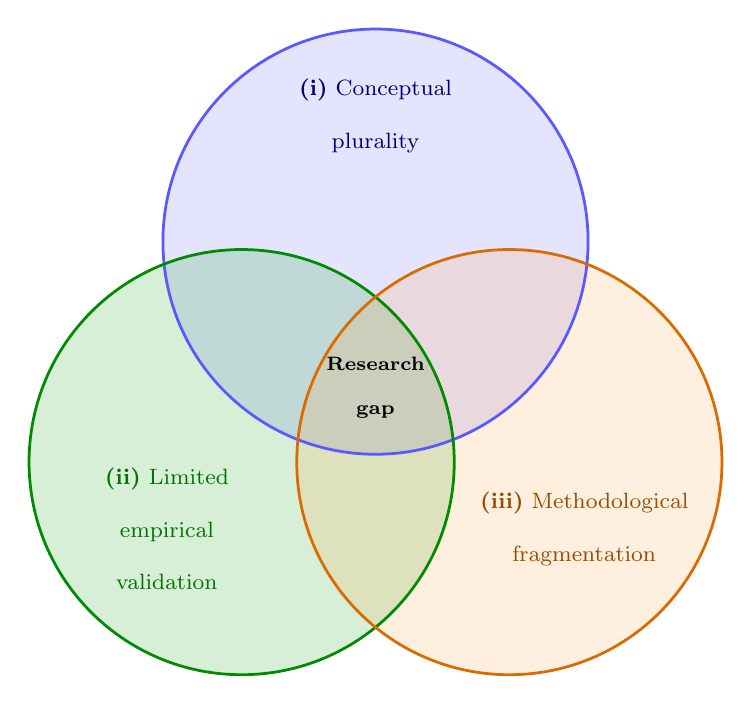
\begin{tikzpicture}[font=\footnotesize]

% ---- three deficit circles ----
\def\R{2.7}
\coordinate (Ci) at (0,1.5);      % (i)  conceptual plurality
\coordinate (Cii) at (-1.7,-1.3); % (ii) limited empirical validation
\coordinate (Ciii) at (1.7,-1.3); % (iii) methodological fragmentation

\begin{scope}[fill opacity=0.16]
  \fill[blue!65]        (Ci)   circle (\R);
  \fill[green!60!black] (Cii)  circle (\R);
  \fill[orange!80]      (Ciii) circle (\R);
\end{scope}
\draw[blue!65,line width=1pt]        (Ci)   circle (\R);
\draw[green!55!black,line width=1pt] (Cii)  circle (\R);
\draw[orange!85!black,line width=1pt](Ciii) circle (\R);

% ---- short labels in the solo lobes ----
\node[blue!45!black,align=center]    at (0,3.1)    {\textbf{(i)} Conceptual\\plurality};
\node[green!45!black,align=center]   at (-2.65,-2.15) {\textbf{(ii)} Limited\\empirical\\validation};
\node[orange!60!black,align=center]  at (2.65,-2.15)  {\textbf{(iii)} Methodological\\fragmentation};

% ---- the gap at the triple intersection ----
\node[align=center,font=\scriptsize\bfseries] at (0,-0.35)
  {Research\\gap};

\end{tikzpicture}
\caption{\textbf{The research gap as the intersection of three deficits.}
Resilience research is held back by three interlocking deficits:
\textbf{(i)} conceptual plurality without operational convergence,
\textbf{(ii)} limited empirical validation of adaptive performance, and
\textbf{(iii)} methodological fragmentation across domains. Each is individually
surmountable; it is their \emph{intersection} that defines the gap this review
targets---resilience can be declared but not evaluated, because the field
simultaneously lacks a shared construct (i), cumulative evidence (ii), and
transferable measures (iii). The Enactment--Scope framework and the agenda of
Section~\ref{sec:RD} are organized to close that overlap.}
\label{fig:venn_gaps}
\end{figure}


\textbf{Conceptual plurality without operational convergence:} Organizations must demonstrate resilience using a single vocabulary, but the literatures behind that term specify incompatible success criteria. Resilience has been conceptualized as mechanical stability, ecological transformation, cognitive adaptability, and socio-technical emergence (Appendix~\ref{appendix:A}). Each tradition is rigorously developed; none is interchangeable. Restoration of predefined functions, regime shift, endurance under stress, and distributed coordination imply different design choices, metrics, and accountabilities.\\

In practice, the trouble follows from what those incompatible criteria require. Each tradition specifies a different answer to what must be preserved, what counts as success, and which interventions belong in scope. When all are folded into one organizational label, boards, regulators, and managers can each pursue a different version of resilience while using the same word---investing in continuity and control where another account demands reconfiguration and learning. Without a shared baseline, neither targets nor metrics can be fixed; resistance, robustness, recovery, agility, and adaptation then circulate as interchangeable terms even though they imply distinct mechanisms and time horizons. The result is definitional drift: resilience is declared in strategy documents, audits, and compliance templates \autocite{hillmann2021organizational} while adaptive capability is built---and evaluated---under separate criteria. Semi-structured interviews with 18 cybersecurity and risk professionals (Appendix~\ref{appendix:C}) show how that drift is enacted: baseline metrics remain elusive (\textit{``\QuoteQuantAmb{}''}), boards request KPIs that are hard to define and fund (\textit{``\QuoteFlexPrec{}''}), and compliance investment is approved more readily than operational adaptation (\textit{``\QuoteCompliance{}''}). Conceptual richness has not yielded operational precision.\\
\\
\textbf{Limited empirical validation and longitudinal grounding:} organizations are assessed on preparedness artifacts at a point in time, not on adaptive performance observed under disruption---let alone its trajectory across successive events. In cybersecurity and risk management, resilience is most often inferred from audits, maturity models, certifications, and control inventories \autocite{power1999audit,skopik2016problem,calder2021iso}. Those instruments have strengthened accountability \autocite{bcbs2021operational,european2022regulation}, yet they certify documented readiness more readily than reconfiguration, improvisation, or learning during live incidents \autocite{woods2015four}. The stakes are not abstract: breaches and intrusions often persist undetected for long intervals before discovery \autocite{bilge2012before,roumani2022detection}, and reviews of organizational resilience find the construct widely invoked with little longitudinal evidence of how firms adapt across repeated shocks \autocite{kruk2017building,barasa2018what}.\\

Regulatory convergences---DORA \autocite{european2022regulation}, NIS2 \autocite{european2022nis2}, FINMA operational-resilience guidance \autocite{finma2023operational}, Basel principles \autocite{bcbs2021operational}, ISO~22301 business continuity management \autocite{calder2021iso}, ISO/IEC~27001 information-security management \autocite{iso27001}, and NIST CSF~2.0 \autocite{nist2024csf}---together with business continuity plan testing, red-teaming, and sector exercises \autocite{ecb2018tiber,enisa2024cybereurope}---have made resilience auditable and exerciseable. Finance and other regulated sectors now treat BCPs, business impact analyses, impact tolerances for important business services, and ICT continuity policies as the operational backbone of preparedness \autocite{bcbs2021operational,european2022regulation}. What they still validate weakly is behavior when disruption departs from script: cross-functional reorganization, informal escalation, ecosystem coordination, and durable post-incident learning \autocite{boin2013resilient}. Field interviews match that limit: exercises can decouple from practice (\textit{``\QuoteCyberRange{}''}), and lessons from incidents rarely persist (\textit{``\QuoteLearning{}''}).\\

To locate the same pattern in the research base, we classified 76 publications by methodological approach and coordination scope (Table~\ref{tab:ResearchGaps}). Simulation, network analysis, and trace-based measurement concentrate at the infrastructural scope, where engineering and complex-systems traditions provide quantitative recovery and cascade dynamics \autocite{bruneau2003framework,francis2014metric,gao2016universal}; the organizational and ecosystem scopes lean instead on case studies, conceptual frameworks, and standards \autocite{vogus2007organizational,burnard2011organisational,linkov2013resilience,bjorck2015cyber}. Methodological fragmentation across scopes, rather than scarcity within any one scope, is the pattern that motivates the agenda developed in Section~\ref{sec:RD}.\\
\\
\begin{center}
\newgeometry{top=.15cm, bottom=2cm, left=2.3cm, right=2.3cm}
\singlespacing
\begin{landscape}
\tiny
\begin{longtblr}[
  caption = {\textbf{Classification of Resilience-related Publications.} This table provides the classification of 89 relevant, impactful and supporting publications associated with resilience according to their corresponding topic/-s and used methodology/-ies. This table allows to extract the key research gaps, where no publication was found (red cells) or only very few (orange cell). Topic-methodology intersections in grey show other research that are less relevant for this research.},
  label = {tab:ResearchGaps}
]{
  width=\linewidth,
  colspec={|Q[1.5cm] Q[1.7cm]|Q[2.6cm] Q[2.6cm] Q[2.6cm] Q[2.6cm] Q[2.6cm] Q[2.6cm] Q[2.6cm]|},
  rowhead = 2,
  hlines, vlines
}
\SetCell[r=2, c = 2]{l} \vspace{2em}\par \textit{Topics}& & \SetCell[r = 1, c = 7]{halign = l}{\textit{Methodologies}} \\
& & \textbf{\makecell{Simulation \\ \& \\ Modeling}} & \textbf{\makecell{Network \\ Analysis}} & \textbf{\makecell{Markers \\ \& \\ Metrics}} & \textbf{\makecell{Technology}} & \textbf{\makecell{Case Studies}} & \textbf{\makecell{Longitudinal \\ Studies}} & \textbf{\makecell{Surveys}} \\
\hline
% === Example block start ===
\SetCell[r=1, c=2]{l}{\textbf{\makecell{Complex Adaptive Systems}}} & &  \SetCell[r=1, c = 1]{l} {\cite{holling1973resilience} \\ \cite{gao2016universal} \\ \cite{pumpuni2017resilience} \\ \cite{krakovska2023resilience}} & \SetCell[r=1, c = 1]{l}{\cite{albert2000error} \\ \cite{bodin2009role} \\ \cite{gao2016universal} \\ \cite{pumpuni2017resilience}} & \SetCell[r=1, c = 1]{l} {\cite{anderies2004framework} \\ \cite{sundstrom2014transdisciplinary} \\ \cite{pumpuni2017resilience}} & \SetCell[r=1, c = 1]{bg = gray!50} & \SetCell[r=1, c = 1]{l} {\cite{ostrom1990governing} \\ \cite{lanzara1999transient} \\ \cite{folke2004regime} \\ \cite{weick2011managing}} & \SetCell[r=1, c = 1]{bg = gray!50} & \SetCell[r=1, c = 1]{l}{\cite{ostrom1990governing} \\ \cite{levin1998ecosystems} \\ \cite{gunderson2002panarchy} \\ \cite{walker2004resilience} \\ \cite{heinimann2017infrastructure}}\\
\hline
\SetCell[r=1,c=2]{l}{\textbf{\makecell{Engineering}}} & & \SetCell[r=1, c = 1]{l}{\cite{wiener1948cybernetics} \\ \cite{panteli2017metrics}} & \SetCell[r=1, c = 1]{l}{\cite{albert2000error} \\ \cite{gao2016universal}} & \SetCell[r=1, c = 1]{l}{\cite{bruneau2003framework} \\ \cite{francis2014metric} \\ \cite{panteli2017metrics}} & \SetCell[r=1, c = 1]{l}{\cite{rane2024artificial}} & \SetCell[r=1, c = 1]{l}{\cite{paries2017resilience}} & \SetCell[r=1, c = 1]{bg = gray!50} & \SetCell[r=1, c = 1]{l}{\cite{holling1996engineering} \\ \cite{francis2014metric} \\ \cite{ivanov2022viable}} \\
\hline
\SetCell[r=1,c=2]{l}{\textbf{\makecell{Ecology \& Social Systems}}} & & \SetCell[r=1, c = 1]{l}{\cite{holling1973resilience} \\  \cite{hashimoto1982reliability} \\ \cite{ives1995measuring}} & \SetCell[r=1, c = 1]{l}{\cite{bodin2009role}} & \SetCell[r=1, c = 1]{l}{\cite{ives1995measuring} \\ \cite{sundstrom2014transdisciplinary}} & \SetCell[r=1, c = 1]{l}{\cite{maillart2024computational}} & \SetCell[r=1, c = 1]{l}{\cite{berkes1998linking} \\ \cite{lebel2006governance} \\ \cite{mahajan2022participatory}} & \SetCell[r=1, c = 1]{l}{\cite{maillart2024computational}} & \SetCell[r=1, c = 1]{l}{\cite{folke2010resilience} \\ \cite{leslie2013response}\\ \cite{francis2014metric} \\ \cite{allen2018quantifying}}\\
\hline
\SetCell[r=1,c=2]{l}{\textbf{\makecell{Climate Change \& Disaster Management}}} & & \SetCell[r=1, c = 1]{l}{\cite{dawson2011agentbased} \\ \cite{panteli2017metrics} \\ \cite{aydin2018integration}} & \SetCell[r=1, c = 1]{l}{\cite{jacobs2017applying} \\ \cite{aydin2018integration}} & \SetCell[r=1, c = 1]{l}{\cite{bruneau2003framework}} & \SetCell[r=1, c = 1]{l}{\cite{arnold2004informationsharing} \\ \cite{aerts2018integrating}} & \SetCell[r=1, c = 1]{l}{\cite{dawson2011agentbased} \\ \cite{mahajan2022participatory}} & \SetCell[r=1, c = 1]{l}{\cite{moreno2018womens}} & \SetCell[r=1, c = 1]{l}{\cite{alexander2013resilience} \\ \cite{meerow2016defining} \\ \cite{adger2005socialecological} \\ \cite{leichenko2024climate}}\\
\hline
\SetCell[r=1,c=2]{l}{\textbf{\makecell{Psychology \& Neuroscience}}} & & \SetCell[r=1, c = 1]{l}{\cite{manikis2019computational} \\ \cite{ungar2021modeling}} & \SetCell[r=1, c = 1]{bg = gray!50} & \SetCell[r=1, c = 1]{l}{\cite{mcewen2004protection} \\ \cite{rakesh2019resilience}} & \SetCell[r=1, c = 1]{l}{\cite{klein2008performing} \\ \cite{bada2019cyber} \\\cite{kalisch2024neurobiology}} & \SetCell[r=1, c = 1]{l}{\cite{bada2019cyber}} & \SetCell[r=1, c = 1]{l}{\cite{rutter1987psychosocial} \\ \cite{masten2010disasters}} & \SetCell[r=1, c = 1]{l}{\cite{wagnild1993development} \\ \cite{luthar2000construct} \\ \cite{campbell2007psychometric} \\ \cite{feder2019biology}}\\
\hline
\SetCell[r=1,c=2]{l}{\textbf{\makecell{Public Health}}} & & \SetCell[r=1, c = 1]{l}{\cite{brauer2008compartmental} \\ \cite{luke2012systems}}  & \SetCell[r=1, c = 1]{l}{\cite{luke2012systems}} & \SetCell[r=1, c = 1]{l}{\cite{cutter2010disaster} \\ \cite{kruk2017building}} & \SetCell[r=1, c = 1]{l}{\cite{arnold2004informationsharing}} & \SetCell[r=1, c = 1]{l}{\cite{barasa2018what} \\ \cite{haldane2021health}} & \SetCell[r=1, c = 1]{l}{\cite{gibbs2013beyond} \\ \cite{aase2020resilience}} & \SetCell[r=1, c = 1]{l}{\cite{norris2007community} \\ \cite{barasa2018what}}\\
\hline
\SetCell[r=2, c=1]{l}{\vspace{-16.25em}\par \textbf{Management}} & \SetCell[r=1, c=1]{l}{\textbf{Organizational}} & \SetCell[r=1, c = 1]{bg = red!20} & \SetCell[r=1, c = 1]{bg = red!20} & \SetCell[r=1, c = 1]{l}{\cite{kuypers2018designing}} & \SetCell[r=1, c = 1]{l}{\cite{klein2008performing} \\ \cite{bada2019cyber} \\ \cite{almeida2020challenges}} & \SetCell[r=1, c = 1]{l}{\cite{lanzara1999transient} \\ \cite{westrum2004typology} \\ \cite{weick2011managing} \\ \cite{henfridsson2013generative} \\ \cite{barasa2018what} \\ \cite{bada2019cyber} \\\cite{boh2023building}} & \SetCell[r=1, c = 1]{bg = gray!50} &  \SetCell[r=1, c = 1]{l}{ \cite{westrum2004typology}\\ \cite{teece2007explicating} \\ \cite{vogus2007organizational} \\ \cite{bhamra2011resilience} \\ \cite{burnard2011organisational} \\ \cite{lengnick2011developing} \\ \cite{boin2013resilient} \\ \cite{henfridsson2013generative} \\ \cite{skopik2016problem} \\ \cite{dupont2019cyberresilience} \\ \cite{barasa2018what} \\ \cite{duchek2019organizational} \\ \cite{calder2021iso} \\\cite{hepfer2022heterogeneity} \\ \cite{he2022building}}\\
\cline[dashed]{2-9}
&  \SetCell[r=1, c=1]{l}{\textbf{Risk \& Cyber}} & \SetCell[r=1, c = 1]{bg = red!20} & \SetCell[r=1, c = 1]{bg = orange!20}{\cite{gillard2023efficient}} & \SetCell[r=1, c = 1]{l}{\cite{linkov2013resilience} \\ \cite{panteli2017metrics}} & \SetCell[r=1, c = 1]{l}{\cite{aerts2018integrating} \\ \cite{almeida2020challenges}} & \SetCell[r=1, c = 1]{l}{\cite{lostri2022shared} \\ \cite{boh2023building}} & \SetCell[r=1, c = 1]{l}{\cite{kuypers2018designing}} & \SetCell[r=1, c = 1]{l}{\cite{baselcommittee2011basel} \\ \cite{bjorck2015cyber} \\ \cite{woods2015four} \\ \cite{skopik2016problem} \\ \cite{linkov2019fundamental} \\ \cite{dupont2019cyberresilience} \\  \cite{hausken2020cyber}  \\ \cite{calder2021iso} \\ \cite{lostri2022shared}} \\
\end{longtblr}
\end{landscape}
\end{center}
\restoregeometry



\textbf{Methodological fragmentation and limited transfer:} the analytical tools needed to observe adaptive performance are developed elsewhere, but not where organizational resilience is governed. That distribution, summarized in Table~\ref{tab:ResearchGaps}, is consequential. Without methods that can trace reconfiguration, cascade, and learning under disruption, evaluation defaults to maturity models, expert judgment, and audit documentation \autocite{skopik2016problem,heinimann2017infrastructure}. Field interviews \autocite{rota2024} describe the same pattern organizationally: IT, risk, and compliance often operate in silos with limited cross-functional integration (\textit{``\QuoteSilos{}''}), which blocks analytical tools from entering shared governance routines. Disciplinary silos therefore stall the transfer of advances that could close the empirical deficit above \autocite{abbasi2016big,aerts2018integrating,falco2019cyber}.\\

Even within cybersecurity, formal models of attack--defense dynamics exist, yet they are seldom integrated into broader organizational resilience architectures. Other transferable approaches, including ecological network analysis \autocite{luke2012systems}, transportation recovery modeling, and agent-based infrastructure risk models \autocite{dawson2011agentbased}, also remain underused in digital resilience planning. The field study describes the same decoupling at the tool level: most firms adopt NIST CSF, ISO/IEC~27001, or COBIT selectively rather than as integrated evaluation systems \autocite{rota2024}; a few experiment with Security Operations Center (SOC) ticket histories as resilience proxies, yet analysis remains immature (\textit{``\QuoteSoc{}''}). The problem is therefore not methodological scarcity. It is the weak translation of technical advances in resilience measurement into governance tools that organizations can actually use \autocite{heinimann2017infrastructure,aerts2018integrating}.\\
\\
Transfer across fields is nevertheless precedented. Engineering recovery metrics have entered disaster and infrastructure policy through standardized indicator sets and recovery-time objectives \autocite{bruneau2003framework,cutter2010disaster}. Ecological resilience has been translated into social-ecological adaptation and governance frameworks \autocite{walker2004resilience,folke2010resilience}. Network and simulation methods have migrated into climate risk, transportation recovery, and flood assessment \autocite{dawson2011agentbased,aerts2018integrating}. Public-health research has linked resilience to measurable health-system capacity \autocite{kruk2017building}. Cyber-resilience work offers a partial analogue in its move from engineering metrics to system-level evaluation \autocite{linkov2013resilience,panteli2017metrics,kuypers2018designing}. Supply-chain and digital-organizational studies show the same logic beginning to cross into management under crisis conditions \autocite{ivanov2022viable,boh2023building}. Field interviews suggest that organizational transfer remains at the same early stage: frameworks are localized rather than standardized, indicator work is improvised rather than validated, and simulation-based methods fail to persist in practice when disconnected from daily operations or from organizational memory. The lesson is not that transfer is impossible, but that it requires validated indicators embedded in governance---a step management and cyber-risk research has taken only selectively.\\
\\
The preceding gaps converge on a single, urgent requirement: methods that trace adaptation \emph{over time} in socio-technical systems, not control design captured at a point in time. The stakes of not having them are concrete. Without longitudinal traces, resilience cannot be distinguished from luck, compliance cannot be distinguished from capability, and an organization has no way to know whether each successive incident leaves it stronger, unchanged, or quietly more brittle (Figure~\ref{fig:trace_vs_snapshot}). Maturity scores and audit snapshots certify what was in place, not whether the organization actually adapted---so the field keeps measuring the wrong object, rewarding documentation over demonstrated recovery and allowing failures to recur under the appearance of control. This is therefore not a methodological refinement but a precondition for evaluating resilience at all. Dynamical-systems approaches---basin stability, return dynamics, perturbation--response analysis---already deliver tools for tracing in complex-systems research \autocite{ives1995measuring,gao2016universal,krakovska2023resilience}; their maturity in adjacent fields and their near-absence from the management and cyber-risk cells of Table~\ref{tab:ResearchGaps} is precisely the difficulty to transfer this review sets out to close. For most large organizations today, the distinction between ``organizational'' and ``digital organizational'' resilience is largely analytical rather than empirical: coordination, data, and governance already run through infrastructures and partners that are constitutive of how the firm operates \autocite{henfridsson2013generative,liu2022network,boh2023building}. We retain \emph{digital organizational resilience} as the paper's shorthand for that socio-technical condition---not to claim a separate theoretical domain, but to mark where the deficits above bite in practice. Section~\ref{sec:Enactment-Scope} takes up the integrative task.

\begin{figure}[t]
\centering
\begin{tikzpicture}[>=Stealth, line width=0.9pt, font=\footnotesize]

% ---- axes ----
\draw[->,gray!60] (0,0) -- (13.2,0) node[above left=1pt and 0pt,black]{time};
\draw[->,gray!60] (0,0) -- (0,5.2) node[above,black,align=center]{adaptive\\capacity};

% ---- disruptions: live incidents (red) and simulated probes (audit / red-team, gray) ----
% D1 probe (x=3), D2 incident (x=5.2), D3 probe (x=7.4)
\foreach \x in {3,5.2,7.4} { \draw[gray!35,dotted] (\x,0.1) -- (\x,4.7); }
\node[gray!75,font=\scriptsize,align=center] at (3,-0.45)   {audit /\\red-team};
\node[red!70!black,font=\scriptsize,align=center] at (5.2,-0.45) {live\\incident};
\node[gray!75,font=\scriptsize,align=center] at (7.4,-0.45) {red-team};
\node[gray!85,font=\scriptsize] at (3,4.95) {\scriptsize(simulated disruption)};

% disruption markers on the axis
\node[gray!75] at (3,0.0)   {\scriptsize$\triangledown$};
\node[red!70!black] at (5.2,0.0) {\scriptsize$\blacktriangledown$};
\node[gray!75] at (7.4,0.0) {\scriptsize$\triangledown$};

% ---- trajectories: all dip at every disruption (real OR simulated); recovery differs ----
% green: monitoring + systematic learning -> each shock converted into a net gain
\draw[green!55!black]
  (1.8,3)--(3,3)--(3.2,2.3)--(4.0,3.5)--(5.2,3.5)--(5.4,2.8)--(6.2,4.0)--(7.4,4.0)--(7.6,3.3)--(8.4,4.6)--(9.6,4.75);
% blue: responds to every probe and incident, recovers to baseline, learns nothing lasting
\draw[blue!45!black]
  (1.8,3)--(3,3)--(3.2,2.3)--(4.0,3.0)--(5.2,3.0)--(5.4,2.3)--(6.2,3.0)--(7.4,3.0)--(7.6,2.3)--(8.4,3.0)--(9.6,3.0);
% red: no learning loop -> each shock leaves less capacity than before
\draw[red!75!black]
  (1.8,3)--(3,3)--(3.2,2.3)--(4.0,2.6)--(5.2,2.6)--(5.4,1.9)--(6.2,2.3)--(7.4,2.3)--(7.6,1.6)--(8.4,1.9)--(9.6,1.6);

% ---- mechanism annotations on the curves ----
\node[green!50!black,font=\scriptsize,align=center] at (6.0,4.75) {monitor + learn:\\each probe/incident\\becomes a gain};
\draw[green!50!black,->] (6.0,4.45) to[bend right=10] (5.7,3.95);
\node[red!65!black,font=\scriptsize,align=center] at (6.55,1.25) {no learning loop:\\lessons lost,\\capacity erodes};
\draw[red!65!black,->] (6.55,1.55) to[bend left=10] (6.1,2.25);

% ---- endpoint labels (outcome): all recover, but to different levels ----
\node[green!55!black,right,font=\scriptsize,align=left] at (9.6,4.75) {recovers\\\emph{stronger}};
\node[blue!45!black,right,font=\scriptsize,align=left]  at (9.6,3.0)  {recovers to\\baseline};
\node[red!75!black,right,font=\scriptsize,align=left]   at (9.6,1.6)  {recovers\\\emph{weaker}};

% ---- early ambiguity note ----
\node[align=center,font=\scriptsize] at (1.05,1.5)
  {one probe is\\ambiguous: all three\\dip and recover\\alike at first};
\draw[->,gray] (1.05,2.15) -- (2.55,2.92);

% ---- brace: longitudinal window ----
\draw[decorate,decoration={brace,amplitude=5pt,mirror},gray!70]
  (2.6,-1.05) -- (9.5,-1.05)
  node[midway,below=4pt,black,font=\scriptsize]
  {longitudinal tracing across disruptions: divergence becomes observable};

\end{tikzpicture}
\caption{\textbf{Monitoring and systematic learning are what separate the
trajectories.} Disruptions are both real (live incidents) and simulated
(audits, certifications, red-team exercises); all are probes that every
organization dips under and recovers from, so any single probe is ambiguous.
All three \emph{recover} after each disruption; what differs is the level they
recover to. Where monitoring feeds a systematic post-incident learning loop,
each shock is converted into a net gain and the organization recovers
\emph{stronger} (an antifragile path); where it responds but institutionalizes
nothing, it recovers only \emph{to baseline} (engineering-style robustness, no net
change); and where no learning loop exists, lessons are lost and it recovers
\emph{weaker}, growing progressively more brittle. Only tracing the loop across
successive disruptions makes the difference---and thus resilience versus luck,
capability versus compliance---observable.}
\label{fig:trace_vs_snapshot}
\end{figure}

>>>>>>> 5962c492beeeeff7385c8b177888710a79b39489
